\section{Design}

Whereas recent work views user threads as a fundamental language abstraction that can
be used to implement preemptible functions, we argue just the opposite.  As discussed
in Section~\ref{sec:intro}, we believe there are already a number of clear use cases
for preemptible functions in their own right, many of which are unrelated to
parallelism and therefore have no need for the scheduler, multiple kernel threads, or
synchronization to support a full threading abstraction.  To prove that our
abstraction does not compromise on expressive power, we end this section by
demonstrating how it can be trivially applied to convert an existing cooperative
userland threading library to a preemptive one.

\begin{figure}
\begin{verbatim}
struct linger {
  bool is_completion;
  union {
    void *completion;
    opaque_t continuation;
  };
};

typedef void *(*function_t)(void *);

struct linger launch(function_t func,
  uint64_t time);
  void *args);
void resume(struct linger *timed_func,
  uint64_t time);
\end{verbatim}
\caption{Core libinger (C language) interface}
\label{fig:interface}
\end{figure}

We propose an interface consisting of two functions, \texttt{launch()} and
\texttt{resume()} (Figure~\ref{fig:interface}).  Both are ordinary, structured calls
whose invocation adheres to C's standard stack discipline; there is no
continuation-style or unstructured control flow.  Client code creates a preemptible
function by passing an ordinary function (or closure) to the \texttt{launch()}
function along with an execution time cap (in microseconds).  If the function
completes on time, \texttt{launch()} propagates its result to the caller; otherwise,
it returns an opaque continuation object that the caller may later pass to
\texttt{resume()} to continue executing the function from wherever it was preempted.
Figure~\ref{fig:usage} shows a basic usage example where the caller is obligated to
perform some work after a certain amount of time (say, call a watchdog), but first
calls into some helper code with weak time bounds.  Thanks to preemptible functions,
the caller doesn't have to trust the helper to know that the watchdog will be called
in time.

\begin{figure}
\begin{verbatim}
res = launch(helper, TIMEOUT, NULL);
call_watchdog(); // Won't be delayed.
if(res.is_completion)
  // We're already done.
  return res.completion;
else
  // Give helper() some more time.
  resume(&res, TIMEOUT);
// ...
\end{verbatim}
\caption{Basic libinger usage example}
\label{fig:usage}
\end{figure}

Although the interface we propose bears some similarities to that of Scheme
engines~\cite{haynes:iucs1984}, some of our design decisions deliberately differ from
theirs:  (1) We return a structured type instead of a function, since the latter
approach would be unportable between languages.  Note that in languages with operator
overloading, it's possible to achieve the other syntax by defining the
\texttt{linger} type's function-call operator to call the \texttt{resume()} function.
(2) Because the preemptible function itself may state, we make the \texttt{linger}
type stateful as well, allowing \texttt{resume()} to mutate it in place.
(3) Instead of passing the preemptible function's return value to a separate callback
function, we return it directly from \texttt{launch()}.  This decision was made
because many modern languages have first-class tagged union (sum) types that allow
the compiler to enforce that the caller explicitly checks whether the function
completed and only accesses the appropriate side of the union.  In addition to the
barebones C interface, our current implementation provides a Rust interface
demonstrating many of these extensions.

Those familiar with futures may notice their applicability to preemptible functions
and simularity to our interface.  While each language's futures differ slightly,
preemptible function bindings can be constructed in the following trivial manner:
To create a new preemptible future, the bindings should call \texttt{launch()} with a
budget of 0 $\mu$s.  Each attempt to poll the future for a value should resolve to a
call to \texttt{resume()} with the timeout passed to poll (if allowed by the
language's API), or else previously associated with the future by other means.

The rest of this section describes the implementation of a novel open-source software
stack supporting preemptible functions and fine-grained userland preemptive
threading.  We start by discussing \textit{libgotcha} (Section~\ref{sec:libgotcha}),
a library that seeks to automatically address many problems related to shared state
in third-party code.  Next, we give an aside illustrating the straightforward
application of libgotcha to provide POSIX async-signal-safety in places where it
wouldn't otherwise exist (Section~\ref{sec:statefulness}).  We then cover the
\textit{libinger} library for running preemptible functions
(Section~\ref{sec:libinger}) and its interaction with libgotcha.  Finally, we present
our experience with porting a userland threading library to libinger in order to make
it preemptive (Section~\ref{sec:threading}).  Figure~\ref{fig:architecture} shows
these components in the overall architecture.

\begin{figure}
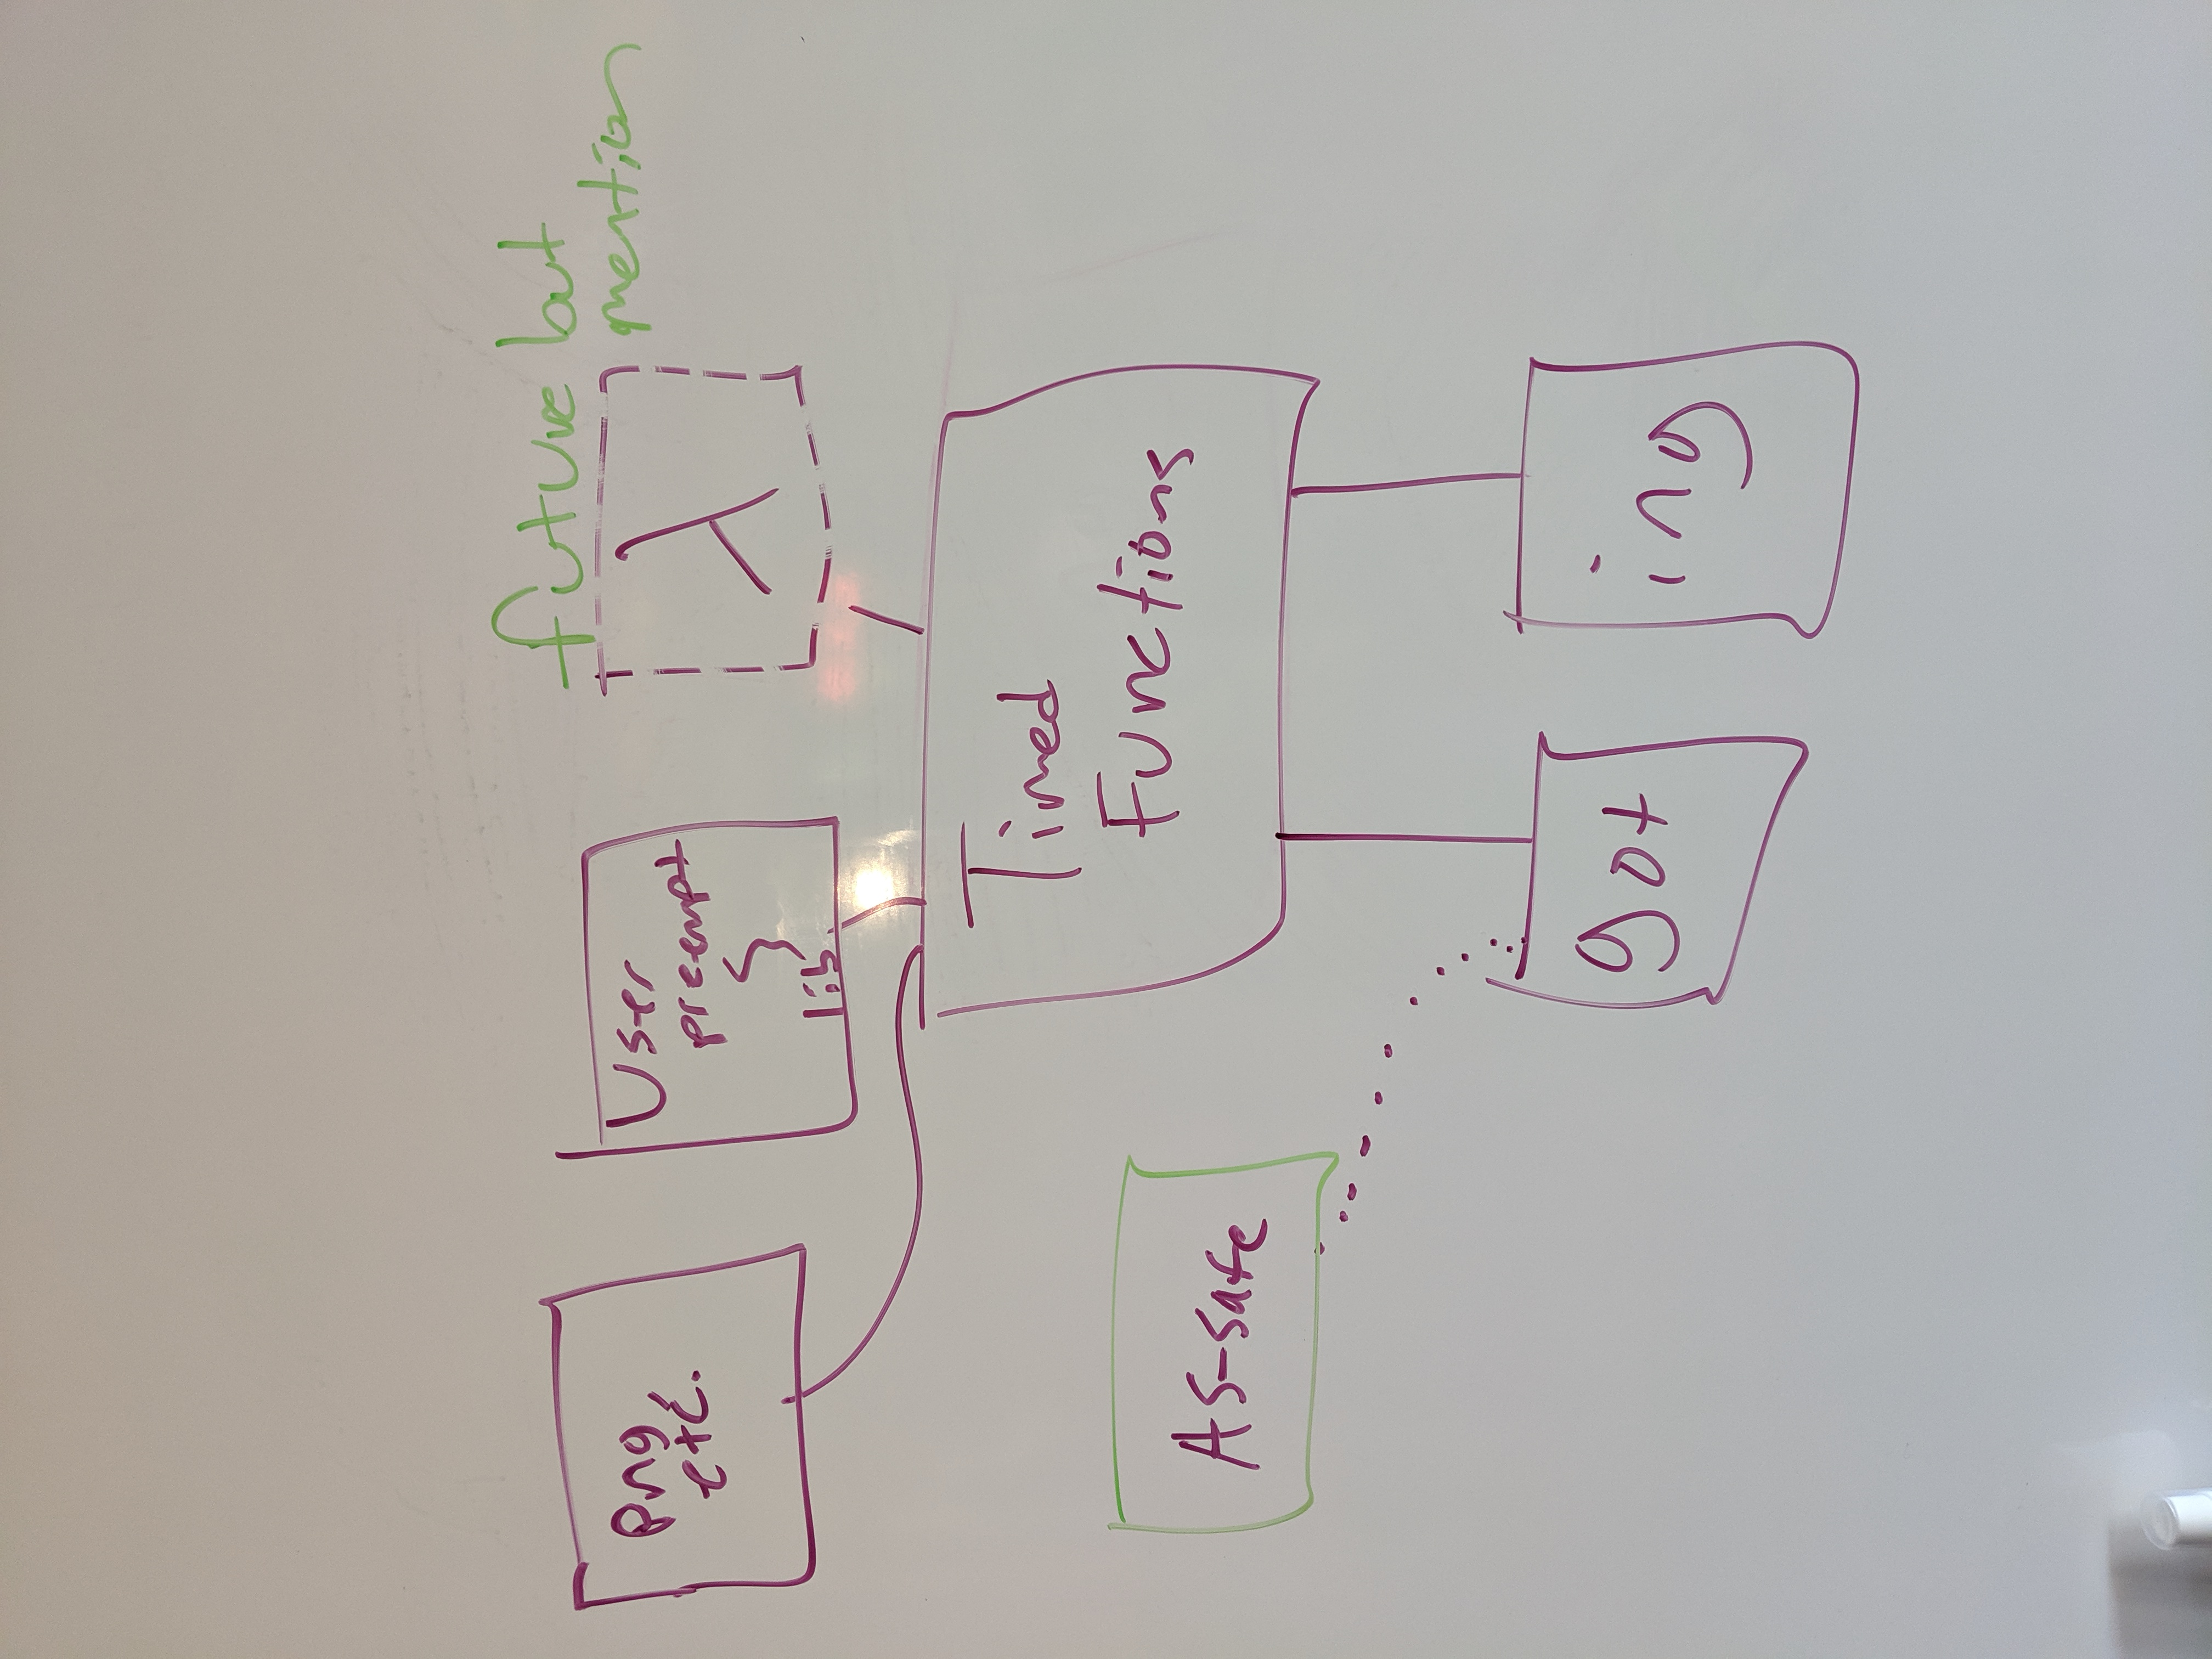
\includegraphics[height=\columnwidth,angle=270]{figs/architecture}
\caption{Architecture of preemptible functions stack}
\label{fig:architecture}
\end{figure}

\subsection{Shared state: \textit{libgotcha}}
\label{sec:libgotcha}

Although shared state is always a problem for preemptible functions, we classify code
that relies on shared state depending on its location:\@ we term it \textbf{internal
stateful code} if it is part of a project (i.e., in the same linked object file)
that uses preemptible functions, and \textbf{external stateful code} otherwise (e.g.,
as is the case for third-party libraries).  Recall that one of our goals is to
support third-party libraries without needing to recompile them.

We begin by briefly discussing internal stateful code.  Figure~\ref{fig:bug} shows
a code passage with a concurrency bug:\@ because the \texttt{timed()} function does
not use an atomic increment operation, its \texttt{launch()} invocation might be
preempted after reading the \texttt{count} variable but before writing it, in which
case the \texttt{resume()} will preserve the existing value of \texttt{1}, causing
the assertion to fail.  We take the stance that internal stateful code is responsible
for implementing its own concurrency control to fix this kind of problem, since the
developers are aware they are using preemptible functions, and therefore (hopefully)
are also aware of the concurrency implications.  If the internal stateful code is
written in Rust instead of C, the compiler can statically prevent many such bugs by
forcing the user to use atomics or locks to protect shared variables such as
\texttt{count}.

\begin{figure}
\begin{verbatim}
static int count = 0;

static void *timed(void *ignored) {
  ++count;
}

int main(void) {
  struct linger res =
    launch(timed, VERY_SHORT, NULL);
  ++count;
  resume(&res, LONG_ENOUGH);
  assert(count == 2); // BUG!

  return 0;
}
\end{verbatim}
\caption{Concurrency bug in internal stateful code}
\label{fig:bug}
\end{figure}

The problem we do have to handle is external stateful code, since there's no way an
existing piece of code can be expected to know that it might be called from a
preemptible function.  In other words, the developers of libraries such as
\texttt{libc} should not need to know that preemptible functions exist.  On the other
hand, we cannot restrict programs that use preemptible functions to calling only
async-signal-safe functions.  This is where libgotcha comes in:\@ it instruments the
boundaries between relocated ELF object files (i.e., executables and dynamic shared
objects).

To avoid both limitations, we slightly weaken the guarantees of either dynamic
linking or preemption, depending on the scenario.  In the common case, we weaken the
property that every use of a dynamically-linked function or global variable resolves
to the same address:\@ we open multiple copies of the shared objects required by the
application, and redirect uses of the library's symbols to a separate copy for each
preemptible function.  In this way, we ensure that inconsistent state from a library
used by one preemptible function cannot affect uses of that same library by other
preemptible functions or the broader application.  While this approach works for many
libraries, it is sometimes inappropriate; for instance, using multiple copies of the
dynamic allocator would cause them to manage the same heap with different free lists.
In such cases, we direct all dynamic calls to the same copy of the function and defer
preemption on that thread until the call has completed, in the style of goroutines.
The rest of this section describes the implementation of these two approaches.  Note
that, in principle, libgotcha functions with the unmodified GNU dynamic linker.

\solb{May need to define libset here, and at least need to introduce the current
libset variable.}

\paragraph{Dynamic linking}

A key feature of shared libraries is the ability to replace them between the time an
application is built and when it is executed.  This is enabled by dynamic linking, an
approach by which the static linker delays the relocation of addresses associated
with \textbf{dynamic calls} to functions and \textbf{dynamic references} to global
variables.  Instead of resolving their addresses, the static linker includes a
\textbf{dynamic relocation table} in each output ELF object file describing the
locations of dynamic calls and references, as well as the name of each target symbol.
A component of the C runtime known as the dynamic linker (\texttt{ld.so}) uses this
table to resolve dynamic symbol addresses after the application is loaded.

It's important to realize that, dynamic calls and references are resolved based on
the name of a symbol, which may be ambiguous between multiple libraries; as such, the
the library associated with each dynamic relocation is not determined until runtime.
In fact, a dynamic relocation might even resolve back to the same object file that
contains it; this is most common when a shared library makes an internal reference to
one of its own public interfaces (since the application might replace that public
interface with its own implementation or one from a different library).  The target
of dynamic relocations will become important for our discussion, so we term them as
\textbf{cross-library references} or \textbf{cross-library calls} if the target
symbol ends up being located in a different object file than the use.

\paragraph{GOTs and PLTs}

\solb{Rather than perform relocations directly into the program instructions...}

When a dynamically-linked executable is run, the kernel first passes control to the
dynamic linker, which loads all required shared object files and populates their
respective \textbf{global offset tables (GOTs)}\footnote{It is from these structures
that \textit{lib\textbf{got}cha} gets its name.} with the resolved addresses of any
referenced dynamic symbols.  Once the program is loaded, any dynamic references to
global variables (which correspond to x86-64 instructions of the form
\texttt{mov~\textit{symbol}@gotpcrel(\%rip),~\%\textit{dest}}) look up the target
symbols' addresses in the GOT for the object file containing the referencing code.

Dynamic function calls are slightly more complicated because they can resolve lazily
the first time they are called.  For instance, the instruction
\texttt{call~printf@plt} causes the assembler to generate a corresponding executable
\textbf{Procedure Linkage Table (PLT)} stub function, as shown in
Figure~\ref{fig:plt}.  The first instruction of this stub looks up the address of the
function by checking a corresponding GOT entry; however, initially this contains the
address of the immediately-following \texttt{pushq} instruction!  Thus, on the first
call, the PLT stub pushes a symbol relocation identifier (here, \texttt{0x0}) onto
the stack and calls into the dynamic linker, which resolves the symbol to the
function's real address, memoizes the result by updating the GOT entry, and finally
jumps into the real function.  Subsequent calls to the PLT stub then forward to the
real function after executing only the initial \texttt{jmpq} instruction.

\begin{figure}
\begin{verbatim}
0000000000001030 <printf@plt>:
  1030:  jmpq   *0x2fe2(%rip) <printf>
  1036:  pushq  $0x0
  103b:  jmpq   1020 <.plt>
\end{verbatim}
\caption{Example PLT entry for call to \texttt{printf()}}
\label{fig:plt}
\end{figure}

\paragraph{Intercepting cross-library calls}

\solb{The fact that the PLT transfers control based on a GOT entry makes it easy to
inject our own code when dynamic calls are made.}

\solb{Mention the need to \texttt{mprotect()}?}

The primary objective of the libgotcha library is to maintain multiple copies of each
loaded ELF object file and seamlessly direct each use at the correct one.  The GNU
dynamic linker includes a feature known as namespaces~\cite{dlmopen-manpage},
inherited from Solaris, that allows loading multiple copies of the same object file
at runtime; however, it treats each namespace as a completely independent dependency
graph of loaded objects, with no relationship to any other namespace.  We built
libgotcha on top of namespaces, to which it adds automatic routing of function calls
and variable references between separate namespaces.  We refer to this augmented
namespace as a \textbf{libset}.  Specifically, libgotcha creates a fixed number of
libsets, each of which can be reused as long as no calls into it from the same thread
of execution are allowed to interleave.  In the event that an operation must be
canceled while it is executing within a libset, the namespace can be reinitialized by
closing all its loaded objects, then reopening and reintegrating them.

In order to use the libgotcha library, a program need only link against its shared
library, which contains a constructor that the dynamic linker will invoke as soon as
it has finished loading all the program's library dependencies.  In order to
automatically transfer control between libsets, this constructor alters the program's
GOT entries to defer to libgotcha code whenever dynamic function calls are made.
Unfortunately, it does not want to do this for all dynamic calls because this would
have inconsistent semantics in the case of object files with self-referential dynamic
relocations, since there's no easy way to instrument static calls at runtime.
(Consider how confusing it would be if a shared library making calls to its own
static helper function and its own public function had those calls to different
copies of itself!)  Because there is no easy way to instrument static calls at
runtime, we make the decision to only switch libsets on cross-library dynamic calls.

Before updating any GOT entries, the libgotcha constructor first has to identify
which ones correspond to cross-library calls.  Doing this is a multi-step process:
First, it traverses the relocation table for each loaded object file, cross
referencing each of its relocation entries against the local object file's symbol
table.  If the symbol table doesn't contain a definition matching the relocation
entry's target, it concludes that the relocation must correspond to a cross-library
call.  Otherwise, it checks the address in the GOT entry corresponding to the
relocation entry:  If this address is outside the bounds of the current object file,
it is a cross-library call.  Otherwise, if the address matches the one from the
symbol table entry, it is not a cross-library call, and should be fixed.  The last
case is the trickiest, because the GOT entry probably still refers to the PLT stub
because the symbol hasn't yet been resolved.  In this case, it resolve the symbol
early, update the GOT entry, and recheck whether it resolved to the local definition
to determine whether it is a cross-library call.

Next, the constructor allocates one or more executable pages full of custom PLT-like
stubs, which we refer to as the \textbf{procedure linkage override tables (PLOTs)}.
Each PLOT is associated with a \textbf{shadow GOT} for each namespace:\@ when a
particular PLOT stub is executed, it pushes an index to the stack and calls a
function, \texttt{procedure\_linkage\_override()}, that decides which libset the call
should target, locates the corresponding shadow GOT, and transfers control to the
address listed at the appropriate index in that table.  (Because this function
is injected into the "middle" of function calls, it is written in assembly to avoid
clobbering any of the application's registers.)  The constructor sets this system up
by replacing each GOT entry corresponding to a cross-library call with a fresh PLOT
entry, but storing the previous value in the shadow GOT for the main namespace.  It
then opens another copy of each library in each namespace, redirects its
cross-library calls at the same PLOT stubs, and creates a shadow GOT for each
namespace.

The setup procedure described so far has one significant problem:\@ recall that a PLT
call memoizes the real address of its symbol by replacing the GOT entry, which should
cause subsequent calls to skip libgotcha's \texttt{procedure\_linkage\_override()}
codepath!  In order to prevent this, the constructor updates the relocation entries
corresponding to cross-library calls to point at \textit{shadow} GOT entries.  This
means that memoization still works, as shown in Figure~\ref{fig:override}.

\paragraph{Incercepting cross-library references}

\solb{Mention taking the address of a function}

\solb{Mention COPY relocations and DF\_1\_NODELETE libraries}

\begin{figure}
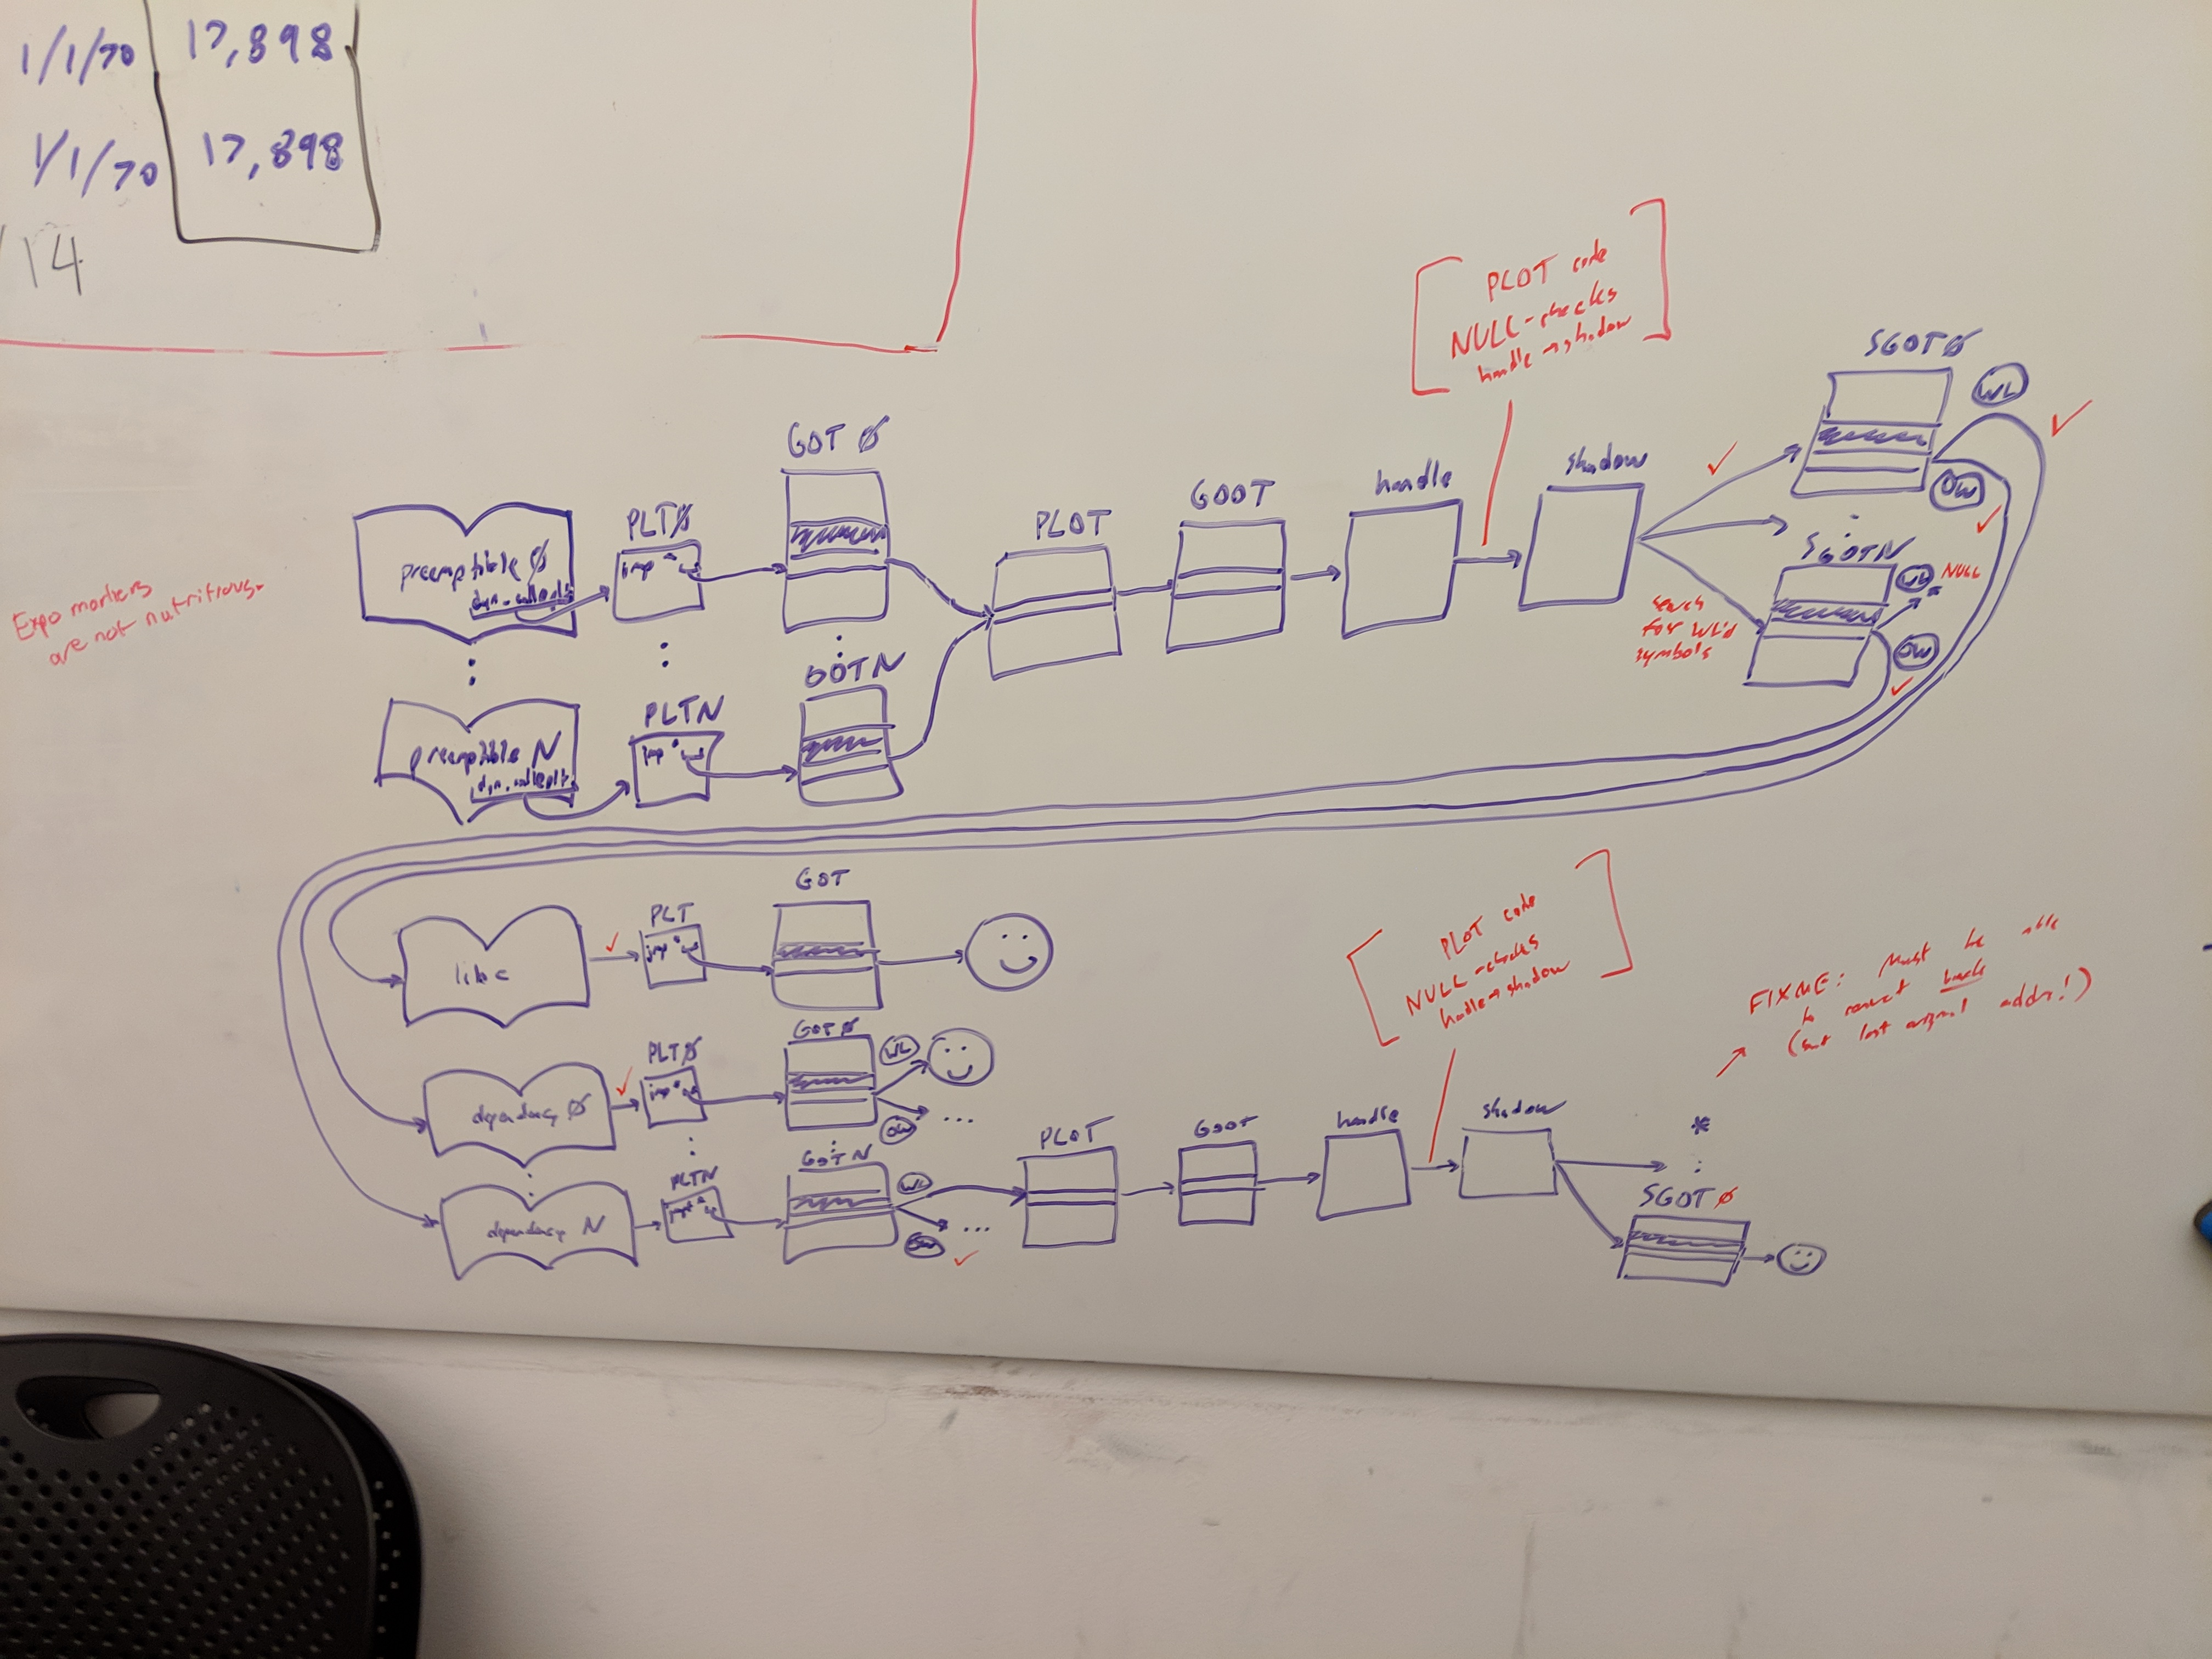
\includegraphics[width=\columnwidth]{figs/tables}
\caption{\texttt{procedure\_linkage\_override()}'s table lookups}
\label{fig:override}
\end{figure}

\subsection{Case study: Establishing AS-safety}
\label{sec:statefulness}

\subsection{Preemptible functions: \textit{libinger}}
\label{sec:libinger}

\begin{figure}
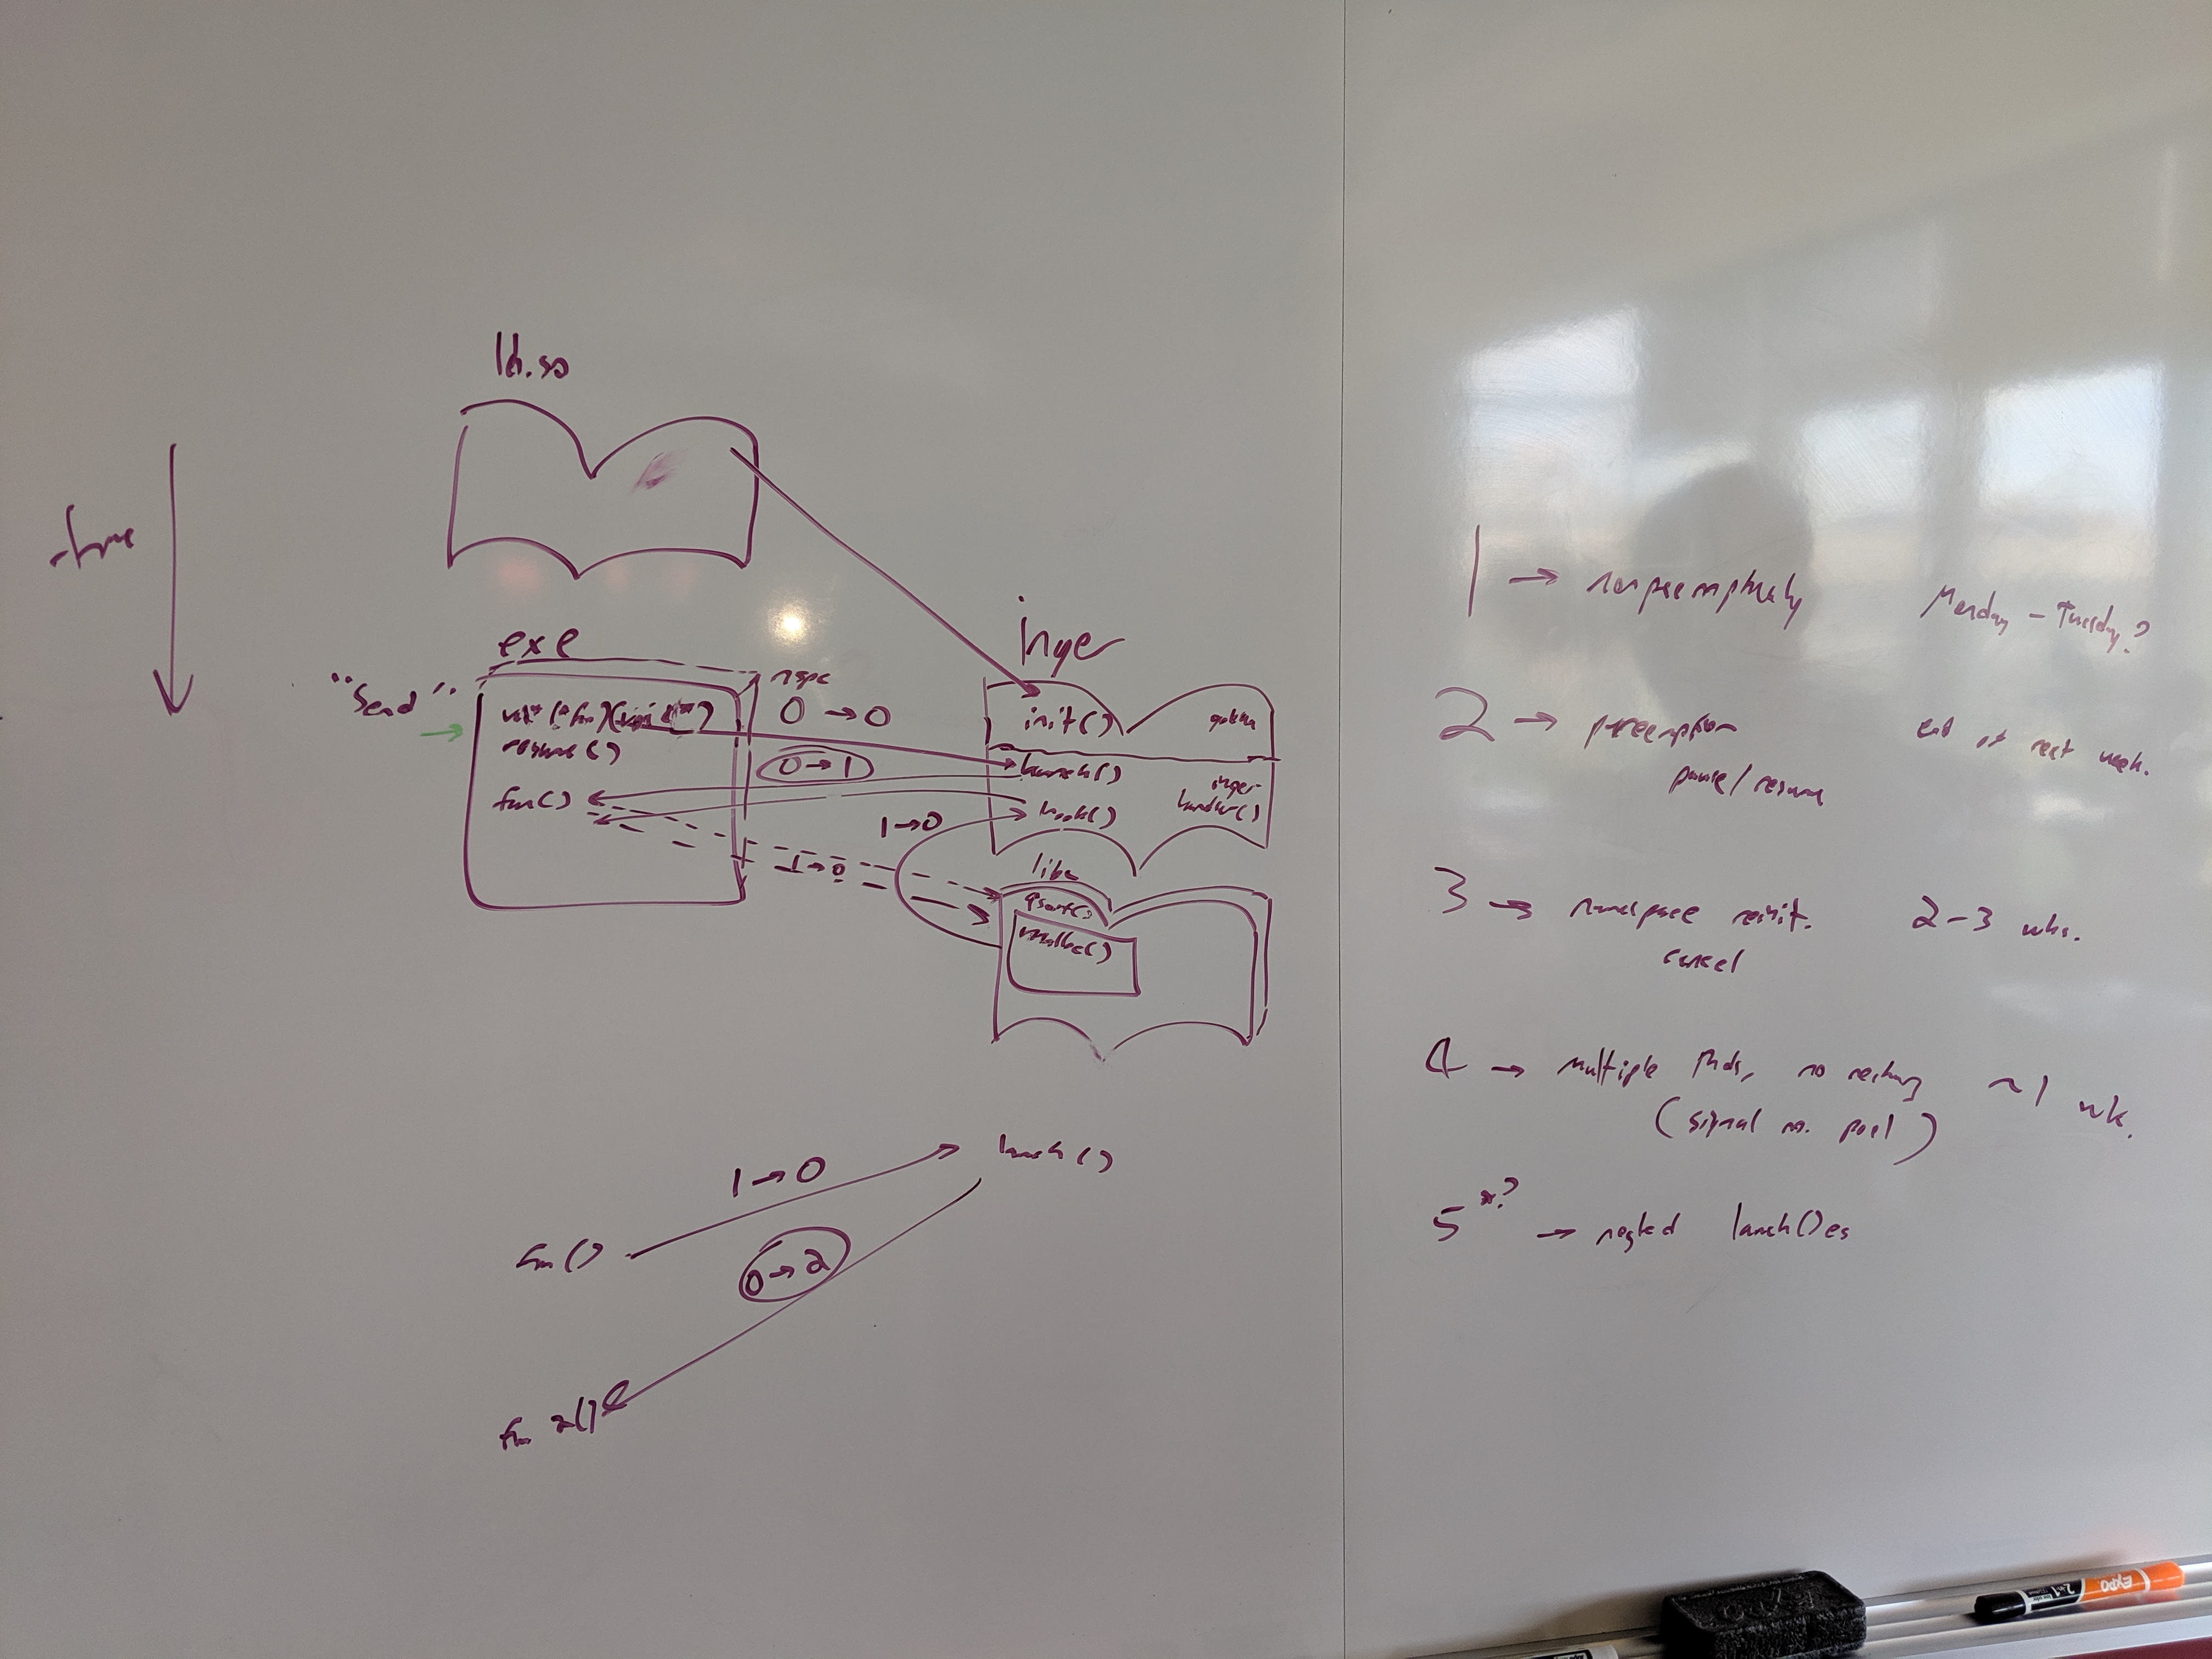
\includegraphics[width=\columnwidth]{figs/calltree}
\caption{How preemptible function dispatch works}
\end{figure}

\subsection{Case study: Userland threading}
\label{sec:threading}

\solb{Discuss Table 1 from Shinjuku and its implications for our design}

\solb{Go ``also'' heap-allocates goroutine locals: \url{https://github.com/golang/go/issues/33216}}
